\documentclass[11pt, oneside]{article}
\usepackage[a4paper,left=2cm,bottom=2.5cm,right=2cm,top=2.5cm,footskip=1cm]{geometry}
\usepackage{amsmath, amsthm}
\usepackage{amssymb}
\usepackage{verbatim}
\usepackage[export]{adjustbox}
\usepackage{fancyvrb}
\usepackage{algpseudocode}
% \usepackage{fontspec}
% \usepackage{fontawesome}
\usepackage{pifont}
\usepackage{array,multirow, rotating}
\usepackage{enumitem}
\usepackage{enotez, multicol}
\usepackage{xcolor}
\setlist[enumerate]{nosep, itemsep=3pt}%, topsep=5pt}
\setlist[itemize]{nosep, itemsep=3pt}%, topsep=5pt}
\renewcommand{\labelitemi}{$\bullet$}
\renewcommand{\theenumiii}{\arabic{enumiii}}
\renewcommand{\labelenumiii}{\theenumiii)}
\usepackage[bottom]{footmisc}
\usepackage{caption, float}
\usepackage{subcaption}
\usepackage{titlesec}
\usepackage{hyperref}
\hypersetup{colorlinks=true, pdfstartview=FitV, linkcolor=blue, citecolor=blue, plainpages=false, pdfpagelabels=true, urlcolor=blue}
\usepackage[all]{hypcap}
\usepackage[extrafootnotefeatures]{xepersian}
\twocolumnfootnotes

\newcolumntype{P}[1]{>{\centering\arraybackslash}m{#1}}
\newcolumntype{C}{>{\centering\arraybackslash}c}
\newcolumntype{R}{>{\centering\arraybackslash}r}


\newcommand{\ev}[2]{#1\endnote{#1\hspace*{\fill}  \lr{#2} \hbox to 0.2\textwidth{}}}

\newcommand{\cross}{\ding{53}}
\newcommand{\tick}{\checkmark}
\newcommand{\sel}{\ding{86}}
\newcommand{\ch}{$\bullet$}

\newcommand{\Ms}{\lr{M}}
\newcommand{\Cl}{\lr{C}}
\newcommand{\Vr}{\lr{V}}
\newcommand{\Rc}{\lr{R}}

\newcommand{\Pb}{\lr{P}}
\newcommand{\Dt}{\lr{D}}

\titlespacing*{\subsection}{0pt}{3pt}{0pt}
\titlespacing*{\section}{0pt}{3pt}{0pt}
\titlespacing*{\subsubsection}{0pt}{3pt}{0pt}

\renewcommand\thesection{\arabic{section}-}
\renewcommand\thesubsection{\thesection\arabic{subsection}-}
\renewcommand\thesubsubsection{\thesubsection\arabic{subsubsection}-}

\setenotez{list-name={\raggedleft\rl{واژه‌نامه}}}
\renewcommand\refname{\raggedleft\rl{مراجع}}

% \AtEveryEndnotesList{\begin{multicols}{2}} % before the whole list
% \AfterEveryEndnotesList{\end{multicols}}   % after the whole list
% \AfterEveryListSplit{\begin{multicols}{2}} % after a sub-heading in the splitted list
% \AtEveryListSplit{\end{multicols}}         % before a sub-heading in the splitted list


\setLTRbibitems
\settextfont[
Scale=1.09,
Extension=.ttf,
Path=fonts/,
BoldFont=XB NiloofarBd,
ItalicFont=XB NiloofarIt,
BoldItalicFont=XB NiloofarBdIt
]{XB Niloofar}

\setlatintextfont[Scale=1]{Times New Roman}
\linespread{1.6}
\newtheorem{proposition}{گزاره}
\newtheorem{theory}{قضیه}
\newtheorem{lemma}{لم}
\newtheorem{corollary}{نتیجه}
\newtheorem{system}{سامانه}

% \setlength{\parindent}{0pt}
\setlength{\parskip}{0.4\baselineskip}
\linespread{1.6}

\let\OLDthebibliography\thebibliography
\renewcommand\thebibliography[1]{
	\OLDthebibliography{#1}
	\setlength{\parskip}{0pt}
	\setlength{\itemsep}{0pt plus 0.3ex}
}

% endnote font for persian vocabs
\defpersianfont\multilingual[Scale=0.9, Extension=.ttf, Path=fonts/]{XB Niloofar}

\DeclareInstance{enotez-list}{custom}{paragraph}
{
notes-sep = -9pt,
format =  \multilingual,
number = \begin{persian} \rl{#1}\end{persian}.
}

\def\enoteformat{\rightskip=0pt \leftskip=0pt \parindent=0.5em \leavevmode\llap{\makeenmark}}


\pagenumbering{gobble}
\begin{document}
	\begin{titlepage}
		\linespread{1.5}
%		\settextfont[Scale=1.2]{B Yas}
%		\setlatintextfont[Scale=1.0]{Times New Roman}
		\centering
		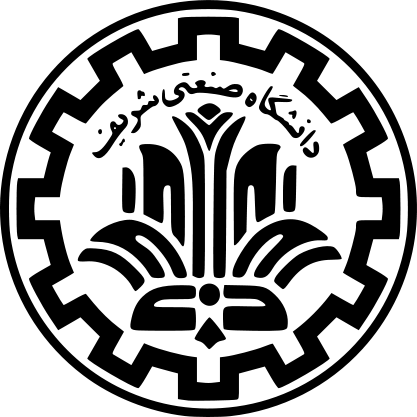
\includegraphics[width=3cm]{sharif-logo.png}\\[\bigskipamount]
		\normalsize	\textbf{دانشگاه صنعتی شریف}\\
		\textbf{دانشکده ریاضی}\\
		\textbf{گزارش سمینار مباحث پیشرفته در الگوریتم‌ها}%
		\\[1.3cm]

		{\LARGE		عنوان:\\
		\textbf{الگوریتم Baruvka برای یافتن درخت پوشای کمینه}\\
		\textbf{\lr{}}\\[2cm]}

		{\Large
		\textbf{نگارش:} \\
		علی توسلی\\
		402201099\\[1.3cm]

		\textbf{استاد درس:}\\
		دکتر زارعی\\[1.3cm]
		\vfill
		\textbf{بهمن 1402}
		}
	\end{titlepage}
	\clearpage
	\pagenumbering{arabic}
	\setcounter{figure}{0}
	\newgeometry{margin=2cm, bottom=2cm}




    \newcommand{\code}[1]{\colorbox{lightgray}{\lr{#1}}}
    \newcommand{\Argmin}[1]{\underset{#1}{\text{argmin}} \hspace{2mm}}
    \newcommand{\Argmax}[1]{\underset{#1}{\text{argmax}} \hspace{2mm}}
    
    \newcommand{\prob}[2][ ]{\mathbb{P}_{#1}\left[#2\right]}
    \newcommand{\expec}[2][ ]{\mathbb{E}_{#1}\left[#2\right]}
    \newcommand{\REF}[1]{\lr{(\ref{#1})}}
    \newtheorem{definition}{تعریف}
    \newtheorem{theorem}{قضیه}
    
    \tableofcontents
    \pagebreak
    \section{پیشگفتار}
    الگوریتم \lr{Baruvka} \cite{c1} قدیمی‌ترین الگوریتم یافتن درخت پوشای کمینه می‌باشد که اولین بار در سال ۱۹۲۶ منتشر شد که روشی بود برای ساختن یک شبکه برق بهینه در شهر مارویای جمهوری چک. در سال ۱۹۳۸ این الگوریتم توسط \lr{Choquet} بازیابی شد. این الگوریتم چند بار دیگر در سال‌های مختلف بازیابی شد که آخرین بار آن در سال ۱۹۶۵ بود توسط \lr{Sollin} که در نهایت هم این الگوریتم به همین نام معروف شد.
    
    از کاربردهای این الگوریتم می‌توان به کاربرد آن در حوزه پردازش موازی اشاره کرد.
    
    \section{شرح مساله}\label{شرح مساله}
    مساله یافتن درخت پوشای کمینه از مسائل معروف و مهم در علوم کامپیوتر می‌باشد. معروف‌ترین الگوریتم‌های این مساله، \lr{Kruskal} \cite{c2} و \lr{Prim} \cite{c3} می‌باشند.

    مساله به این صورت است که یک گراف وزن‌دار بدون جهت داده شده. به دنبال یافتن یک زیردرخت از این گراف هستیم که مجموع وزن یال‌های آن بین همه درخت‌های ممکن کمینه باشد.
    می‌توان گراف را ناهمبند در نظر گرفت، در این صورت به دنبال یافتن یک جنگل پوشای کمینه هستیم.
    
    شکل زیر درخت پوشای کمینه برای یک گراف ساده همبند را نشان می‌دهد. یال‌های پررنگ یال‌های این درخت هستند:
    \begin{center}
        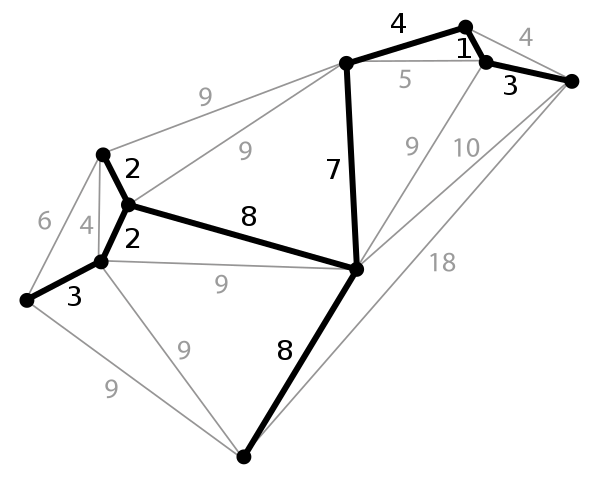
\includegraphics[width=10cm]{resources/mst.svg.png}\\[\bigskipamount]
    \end{center}

    \pagebreak
    \section{الگوریتم}\label{الگوریتم}
    فرض کنید \lr{$V$} مجموعه راس‌های گراف باشد و \lr{$E$} مجموعه یال‌های گراف.

    الگوریتم به این صورت عمل می‌کند که ابتدا هر راس را در مولفه همبندی خودش تعریف می‌کند. در ابتدا مجموعه یال‌های برگزیده شده برای درخت پاسخ مجموعه تهی است و به صورت دوره‌ای
    این مجموعه را کامل می‌کند.
    در هر مرحله، تعداد مولفه همبندی در گراف موجود است که این مولفه‌ها توسط یال‌های برگزیده شده تشکیل شده‌اند.
    در ابتدای هر مرحله، به صورت همزمان، از هر مولفه همبندی، کوچک‌ترین یالی که از آن خارج می‌شود را انتخاب می‌کند.
    سپس این یال‌ها را به مجموعه یال‌های برگزیده اضافه می‌کنیم. این کار را آنقدر انجام می‌دهیم تا به یک درخت پوشا برسیم.

    در ادامه ثابت می‌کنیم این درخت پوشا، کمینه نیز می‌باشد.
    
\subsection{جزئیات الگوریتم}
هنگامی که برای یک مولفه، یال کمینه که از آن خارج می‌شود را انتخاب می‌کنیم، ممکن است چند یال باشند که این خاصیت را داشته باشند.
حال سوالی که پیش‌ می‌آید این است که از بین این‌ها، کدام یال را باید برگزید؟

پاسخ: به این صورت عمل می‌کنیم که مولفه‌ها را شماره‌گذاری می‌کنیم، اگر چند یال بودند که وزن کمینه را داشتند، آن یالی را انتخاب می‌کنیم که مولفه مقصد آن کوچک‌ترین شماره را داشته باشد.
اگر چند یال با خاصیت فوق بودند، یالی را انتخاب می‌کنیم که شماره راس آن کمینه باشد.

\subsection{تحلیل زمانی و حافظه الگوریتم}
\newcommand{\trace}[1]{\mathrm{Tr}\left\{#1\right\}}
به هر عملیات پیدا کردن یال کمینه برای مولفه‌ها، یک گام می‌گوئیم.

\textbf{لم ۱:} تعداد گام‌ها از مرتبه \lr{$O(lg |v|)$} است.

\textbf{برهان:}
در هر گام، تعداد مولفه‌ها حداقل نصف می‌شود (ممکن است در برخی موارد، کمتر از نصف هم بشود). از آنجا که در وضعیت ابتدایی تعداد \lr{$|V|$} مولفه داریم و در حالت انتهایی تنها یک مولفه، بنابراین حداکثر \lr{$O(lg |V|$)} گام خواهیم داشت.
\\
\\
برای هر گام (پیدا کردن کمینه یال خروجی از هر مولفه)، کافی است یک \lr{$DFS$} بزنیم که از مرتبه \lr{$O(|V| + |E|)$} می‌باشد.

بنابراین در مجموع، پیچیدگی زمانی از مرتبه \lr{$O((|V| + |E|) \times lg |V|)$} خواهد بود.

از نظر حافظه، فقط یال‌ها را ذخیره کردیم و در هر مرحله برای هر مولفه یال کمینه آن را نگه داشتیم. بنابراین پیچیدگی حافظه برابر خواهد بود با: \lr{$O(|E| + |V|)$}.

\pagebreak
\section{مثالی از اجرای الگوریتم}
گراف زیر را در نظر بگیرید. می‌خواهیم الگوریتم را روی آن اجرا کنیم. هر عکس نمایانگر یک گام از اجرای الگوریتم یعنی پیدا کردن کمینه یال برای هر مولفه می‌باشد.

گراف ورودی:
\begin{center}
    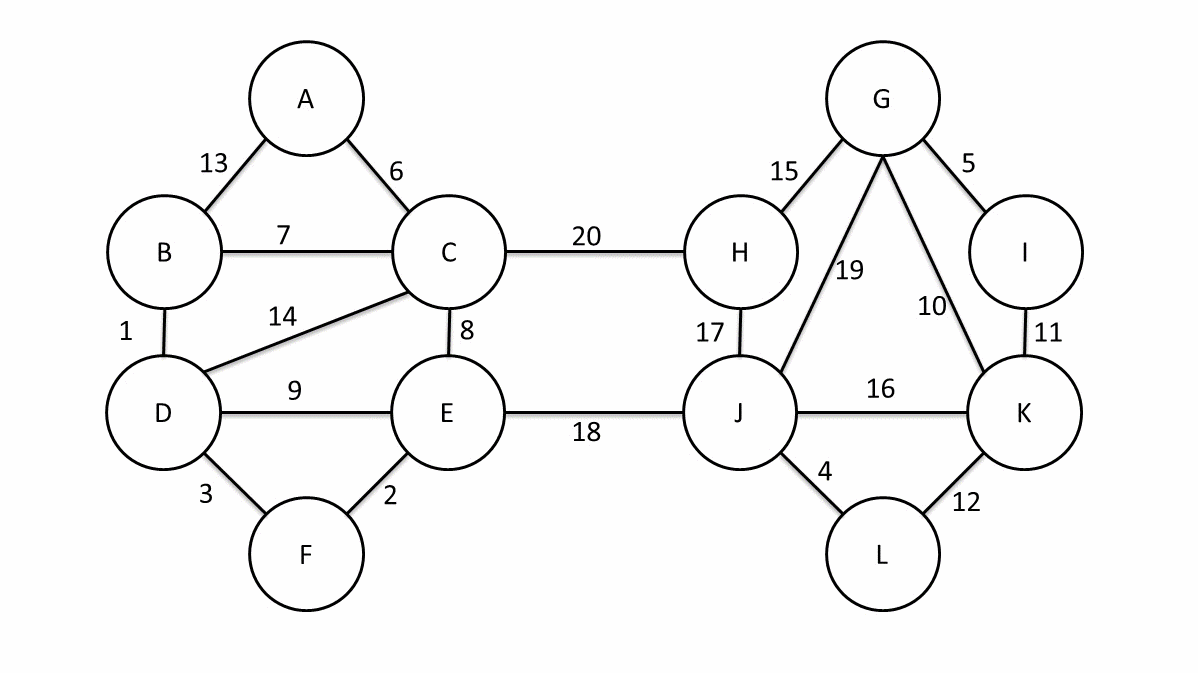
\includegraphics[width=10cm]{resources/input-graph.png}\\[\bigskipamount]
\end{center}

بعد از اجرای گام اول:
\begin{center}
    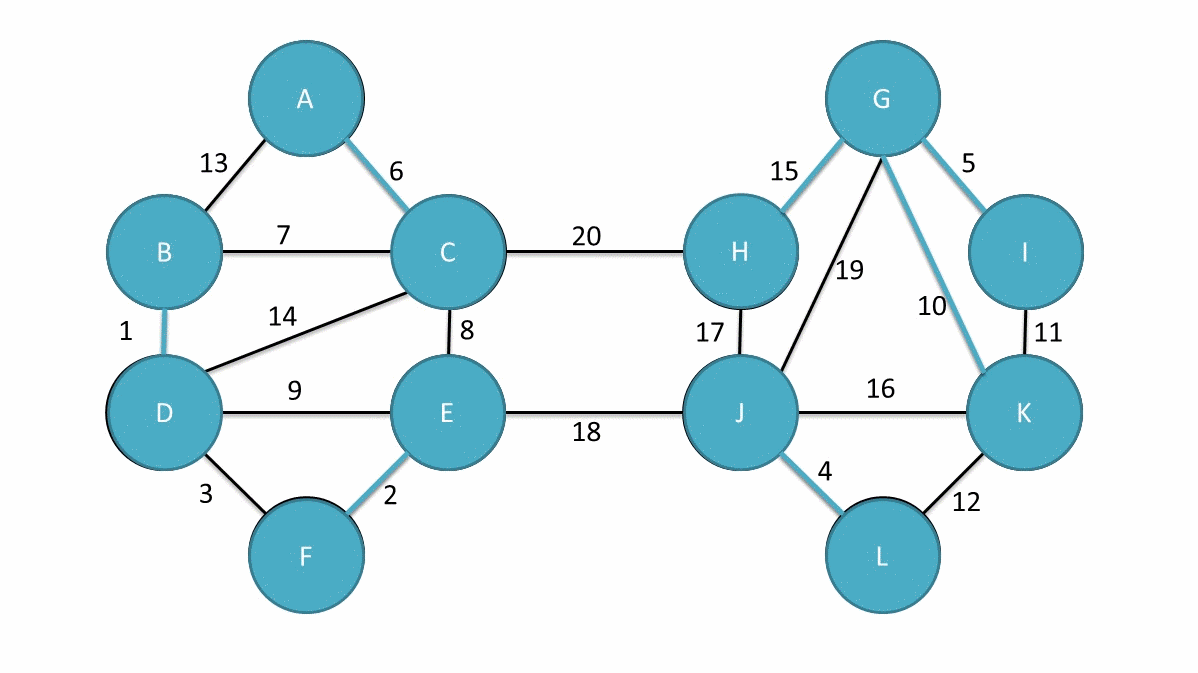
\includegraphics[width=10cm]{resources/step1.png}\\[\bigskipamount]
\end{center}

بعد از اجرای گام دوم:
\begin{center}
    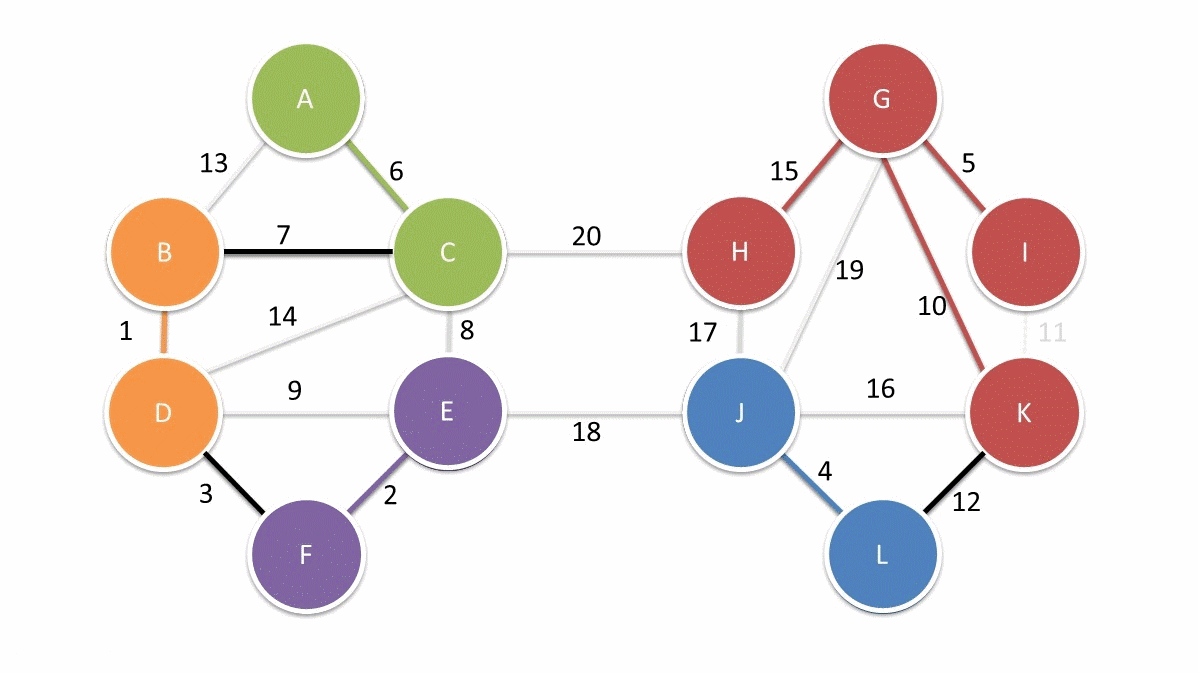
\includegraphics[width=10cm]{resources/step2.png}\\[\bigskipamount]
\end{center}

\pagebreak
بعد از اجرای گام سوم:
\begin{center}
    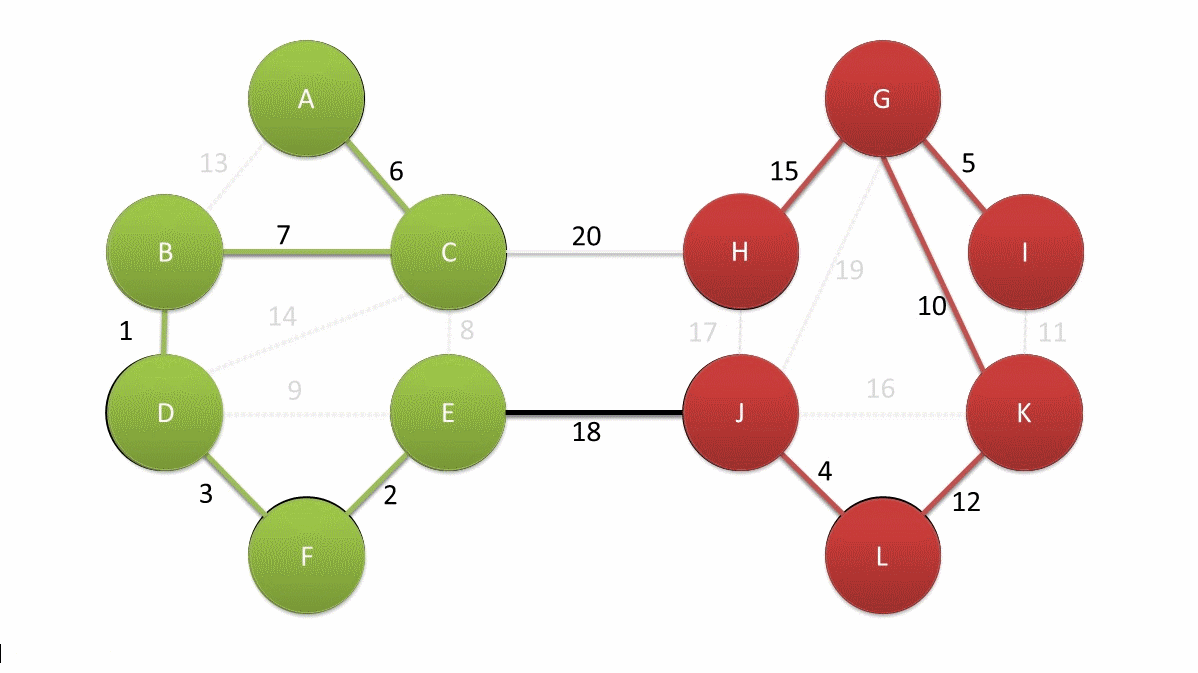
\includegraphics[width=10cm]{resources/step3.png}\\[\bigskipamount]
\end{center}

درخت نهایی:
\begin{center}
    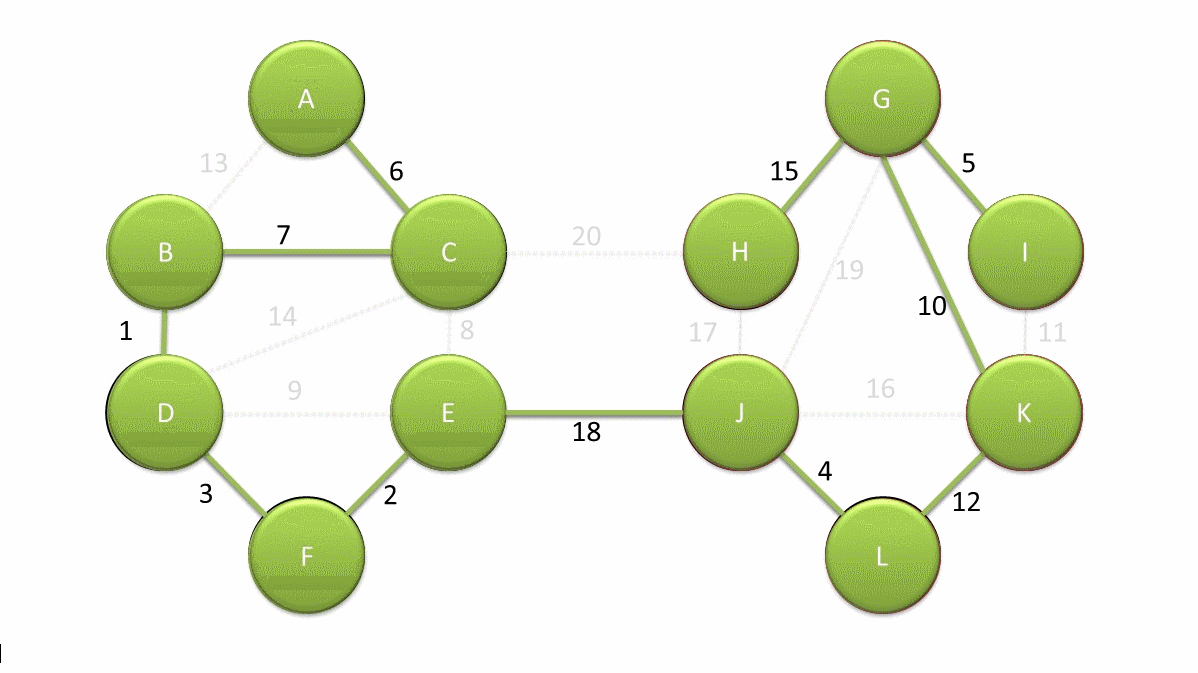
\includegraphics[width=10cm]{resources/output-mst.png}\\[\bigskipamount]
\end{center}

\pagebreak

\section{پیاده‌سازی الگوریتم}
\begin{latin}
    \begin{verbatim}
        Input: A weighted undirected graph G = (V, E)
        Output: F, a minimum spanning forest of G

        Initialize a forest F to (V, E') where E' = {}

        completed := false
        while not completed do
            Find the connected components of F and assign to each vertex its component
            Initialize the cheapest edge for each component to "None"
            for each edge uv in E, where u and v are in different components of F:
                let wx be the cheapest edge for the component of u
                if is-preferred-over(uv, wx) then
                    Set uv as the cheapest edge for the component of u
                let yz be the cheapest edge for the component of v
                if is-preferred-over(uv, yz) then
                    Set uv as the cheapest edge for the component of v
            if all components have cheapest edge set to "None" then
                completed := true
            else
                completed := false
                for each component whose cheapest edge is not "None" do
                    Add its cheapest edge to E'

        function is-preferred-over(edge1, edge2) is
            return (edge2 is "None") or
                    (weight(edge1) < weight(edge2)) or
                    (weight(edge1) = weight(edge2) and tie-breaking-rule(edge1, edge2))
        
        function tie-breaking-rule(edge1, edge2) is
            The tie-breaking rule; returns true if and only if edge1
            is preferred over edge2 in the case of a tie.
    \end{verbatim}
\end{latin}

\pagebreak
\section{درستی الگوریتم}

\textbf{لم ۲:}
در هیچ گامی دور ایجاد نمی‌شود (و بنابراین مستقیم نتیجه می‌شود که در نهایت هم دور ساخته نمی‌شود).

\textbf{برهان:}
فرض کنید در یک گام یک دور ایجاد شود. ابتدا یک فرض اضافه در نظر می‌گیریم و در نهایت ثابت می‌کنیم که این فرض تاثیری نداشته. فرض کنید وزن تمام یال‌ها در گراف اولیه متفاوت باشد.
از آنجا که یال‌ها را بین مولفه‌ها قرار می‌دهیم، کافی است مولفه‌ها را به عنوان \lr{super node} در نظر بگیریم. فرض کنید یک دور ایجاد شده که دنباله آن به این صورت باشد: \lr{$v_1, v_2, ..., v_k, v_1$}. که \lr{$v_i$}ها متمایز هستند و هر کدام نماینده یک مولفه‌ هستند. از آنجا که وزن یال‌ها متمایز است، داریم:
\\
\\
\lr{$w(v_1v_2) < w(v_kv_1)$}
\\
\lr{$w(v_2v_3) < w(v_1v_2)$}
\\
\lr{$w(v_3v_4) < w(v_2v_3)$}
\\
\lr{...}
\\
\lr{$w(v_kv_1) < w(v_{k - 1}v_k)$}

که از این نامساوی‌ها نتیجه میگیریم:

\lr{$w(v_kv_1) < w(v_kv_1)$}

که یک تناقض است. بنابراین در هیچ‌کدام از گام‌ها دور به وجود نمی‌آید. توجه کنید که یک فرض اضافه داشتیم که وزن تمام یال‌ها متمایز است. حال اگر این فرض را حذف کنیم، حتی اگر یکی از تساوی‌ها هم بیشتر اکید باشد باز هم می‌توان همین نتیجه را گرفت. تنها حالت بد این است که همه تساوی‌ها = باشند. در این صورت با توجه به پیاده‌سازی الگوریتم که در صورت مساوی بودن دو یال، یال  با شماره مولفه کمتر را انتخاب می‌کرد به تناقض می‌رسیم.


\lr{$w(v_1v_2) > $}
از آنجا که از هر مولفه تنها یک یال رسم می‌شود، بنابراین یال \lr{$v_1v_2$} باید از مولفه یک انتخاب شده باشد، \lr{$v_2v_3$} باید از مولفه دو باشد و ...
\lr{$w(v_1v_2) < w(v)$}

\textbf{لم ۳:}
درخت نهایی دارای وزن کمینه در بین تمامی درخت‌هاست.

\textbf{برهان:}
ثابت می‌کنیم بعد از هر گام، یک درخت پوشای کمینه وجود دارد که یال‌های فعلی، زیر مجموعه آن باشند.

فرض کنید در یک مرحله، یال \lr(uv) بین دو راس \lr{u} و \lr{v} برگزیده شده.
میخواهیم ثابت کنیم یک درخت پوشای کمینه وجود دارد که این یال بعلاوه یال‌های پیشین را دارد. این کار را به صورت استقرایی انجام می‌دهیم.
فرض کنید مجموعه یال‌های برگزیده قبل از اضافه کردن این یال، \lr{T} باشد. طبق فرض استقرا می‌دانیم یک درخت پوشای کمینه وجود دارد که \lr{T} زیرمجموعه‌ی آن باشد.
اکنون برای اثبات حکم استقرا، کافی است ثابت کنیم یک درخت پوشای کمینه وجود دارد که 
\lr{T + uv} زیر مجموعه آن است.
برهان خلف می‌زنیم. فرض کنید هیچ درخت پوشای کمینه نباشد که این یال‌ها زیرمجموعه آن باشند.
فرض کنید این‌گونه نباشد. یک درخت پوشای کمینه که \lr{T} زیرمجموعه آن است را \lr{M} بگیرید. می‌دانیم یال \lr{uv} در \lr{M} نیست.
پس یک یال دیگری باید باشد که دو مولفه‌ای که \lr{u} و \lr{v} در آن هستند را متصل کنید. این یال را \lr{xy} بگیرید. حال یال \lr{xy} را به \lr{M} اضافه کنید.
واضح است که یک دور ساخته می‌شود.
از طرفی، طبق روشی که در الگوریتم داشتیم، اندازه یال \lr{xy} بیشتر از اندازه \lr{uv} است، زیرا در غیر اینصورت این یال انتخاب می‌شد. بنابراین بعد از اضافه کردن یال \lr{uv}، یک دور ایجاد می‌شود که یال \lr{xy} هم در آن است. حال کافی است یال \lr{xy} را حذف کنیم. واضح است که اندازه درخت کمتر شد و این تناقض است. زیرا فرض کرده بودیم که \lr{M} مجموع وزن کمینه را دارد.

حال اگر دقت کنیم، می‌بینیم که فرض متمایز بودن وزن یال‌ها لازم نبود زیرا می‌توان به یال‌ها مقادیری اضافه کرد که وزن آن‌ها دو به دو فرق کند. اینگونه روند الگوریتم تغییر نمی‌کند ولی اثبات ما کارا خواهد بود. بنابراین لم ثابت شد.
\\
\\
\subsection{جمع‌بندی}
در لم دوم ثابت کردیم هیچ‌گاه دور ایجاد نمی‌شود. از طرفی، در هر گام تعداد مولفه‌های همبندی حداقل یک واحد کم می‌شود.
بنابراین بعد از تعدادی گام حتما به یک درخت می‌رسیم (جایی که تنها یک مولفه همبندی می‌ماند).
از طرفی در لم سوم ثابت کردیم که درختی که بدست می‌آید دارای کمینه وزن است. بنابراین ثابت کردیم که این الگوریتم در نهایت درخت پوشای کمینه را خروجی می‌دهد.

\section{الگوریتم‌های مشابه}\label{الگوریتم‌های مشابه}
همانطور که در بخش اول گفتیم، دو الگوریتم دیگر برای یافتن درخت پوشای کمینه وجود دارند. در جدول زیر به مقایسه این الگوریتم‌ها می‌پردازیم:

\begin{latin}
    \begin{center}
        \begin{tabular}{||c c c c||} 
        \hline
        Algorithm & Time Complexity & Implementation Complexity & Publish Day \\ [0.5ex] 
        \hline\hline
        Baruvka & $O(E \; log \; V)$ & Simple (DFS) & 1926 \\ 
        \hline
        Kruskal & $O(E \; log \; E)$ & Medium (DSU) & 1956 \\
        \hline
        Prim & $O(V + V \; log \; V)$ & Complex (Fibonacci heap) & 1957 \\
        \hline
        \end{tabular}
    \end{center}
\end{latin}






\pagebreak
\linespread{1.0}
\latinfont
\bibliographystyle{ieeetr}
\bibliography{seminar}
\printendnotes[custom]

\end{document}
